
%----------------------------------------------------------------------------------------
%	PART
%----------------------------------------------------------------------------------------

\part{Part 1}

%----------------------------------------------------------------------------------------
%	CHAPTER 1
%----------------------------------------------------------------------------------------

%% \chapterimage{ima2} % Chapter heading image

\chapter{Introduction}


%%\chapterimage{ima2} % Chapter heading image

\chapter{Neuron Dynamics}\

Spiking neural network's neuron model describe how the membrance potential of a neuron change over the time.
In this chapter, we dive into the biological neuron's dynamics and exhibit several examples neuron models in the 
spiking neural network. 

% Beside classical neuron models such as 
% \texttt{Hodgkin-Huxley (HH) model}, \texttt{Leaky integrate-and-fire model}, and \texttt{Zhikevich model},
% we also describe some 

\section{Biological Neuron}\index{Biological Neuron}


\section{Neuron Model Abstract and Taxonomy}\index{Neuron Model Abstract and Taxonomy}
In spiking neural network, Equation~\ref{eq:neuron-state-space-abstract-1} to
Equation~\ref{eq:neuron-state-space-abstract-4} provide a highly abstract description for
 modeling a biological neuron.
In these equation, $\bold x_t$ is the state vector at time $t$, $\Delta x_t$ is the state variation at time 
$t$, $\bold u_t$ is the input vector at time $t$, $V$ is the membrane potential of the neuron, 
$\bold y_t$ is the neuron's output at time $t$, 
and $V_{out}$ is the output voltage that will be sent to the synapses that depature from this neuron. 
$(\bold x_{t})_{i}$ is the $i$-th element of the state vector.

\begin{align}
    \Delta \bold x_t = f(\bold x_t, \bold u_t) \label{eq:neuron-state-space-abstract-1} \\
    \bold y_t = g(\bold x_t, \bold u_t) \label{eq:neuron-state-space-abstract-2} \\
    s.t.,\; (\exists i \in [0, |\bold x_t|])(\bold x_{t})_{i} = V \label{eq:neuron-state-space-abstract-3}\\
            (\exists i \in [0, |\bold y|])_i\bold y = V_{out} \label{eq:neuron-state-space-abstract-4}
\end{align}

These equations are in the form of a \textbf{state-space model (SMM)}.


Equation~\ref{eq:neuron-state-space-abstract-3} indicates that, a neuron should maintain a membrane potential $V$, 
and Equation~\ref{eq:neuron-state-space-abstract-4} indicates that, the neuron's output should contains a 
voltage $V_{out}$.

\subsection{Current-based Neuron}\index{Current-based Neuron}
In a current-based neuron model, the synaptic input is represented as an injected current directly 
added to the membrane potential equation.
we have the input $\bold u_t$ contains the current $I_t$, and $\bold x_t$ contains the membrance potential $V_t$.

We will later to see that a current-based LIF neuron (Section~\ref{sec:current-based-lif}) can hold a form of 
Equation~\ref{eq:current-based-lif-state-space}.


\begin{equation}\label{eq:current-based-lif-state-space}
    \dot V_t = \frac{1}{\tau_m}(-(V_t-V_{rest})+I_t) = f_{CurrentLIF_1}(V_t, \bold u_t = [I_t])
\end{equation}



\subsection{Conductance-based Neuron}\index{Conductance-based Neuron}
In a conductance-based neuron model, the synaptic input is modeled by changing the conductance of the membrane, 
which then affects the current flow.

In the state space representation, the input $\bold u_t$ is the synapse conductance.
let $\bold u_t=g_{syn}(t)$, $\bold x_t = V_t$, we will see that in conductance-based LIF neuron model, it 
hold Equation~\ref{eq:condunce-based-lif-state-space}

\begin{equation}\label{eq:condunce-based-lif-state-space}
    \dot V_t = \frac{1}{\tau_m}(-(V_t-V_{rest})+g_syn(t)(E_{syn}-V_t)) = f_{ConductanceLIF_1}(V_t,  \bold u_t = g_{syn}(t))
\end{equation}




\section{Neuron Model Examples}\index{Neuron Model Examples}
\subsection{Hodgkin-Huxley (HH) Model}\index{Hodgkin-Huxley (HH) Model}

The Hodgkin-Huxley (HH) model is a conductance-based model , which can be utilize to accurately 
reproduce the bio-neuron's dynamics. Its form is shown in Equation~\ref{eq:hh-model-1} to Equation~\ref{eq:hh-model-5}.
Combine all these equations, we get Equation~\ref{eq:hh-model-6}.
% \begin{align} 
% \begin{split}
% P(y=1/x)   &=P(y*>0/x)=P[x\beta+e>0/x]=P[e>-(\beta_{0}+x\beta)/x]\\
% &=1-F[-(\beta_{0}+x\beta)]=F(\beta_{0}+x\beta)
% \end{split}					
% \end{align}

\begin{align}
    I = C_m\frac{dV_m}{dt} + I_{i} \label{eq:hh-model-1} \\
    I_i = I_{Na} + I_K + I_l \label{eq:hh-model-2}  \\
    I_{Na} = g_{Na}(V_m - V_{Na}) \label{eq:hh-model-3} \\
    I_K = g_{K}(V_m - V_{K}) \label{eq:hh-model-4}  \\
    I_l = \bar g_{l}(V_m - V_{l}) \label{eq:hh-model-5} 
\end{align}

\begin{equation}\label{eq:hh-model-6}
    I_l = C_m\frac{dV_m}{dt} + g_{Na}(V_m - V_{Na}) + g_{K}(V_m - V_{K}) + \bar g_{l}(V_m - V_{l})
\end{equation}

Ion channel function $g_{\cdot}$ are function respect to time $t$ and membrance potential $V$.
Specifically, Equation~\ref{eq:hh-model-7} is held.

\begin{equation}\label{eq:hh-model-7}
    g_{Na} = \bar g_{Na}m^3h \\
    g_{K} = \bar g_{K}n^4 \\
    g_{l} = \bar g_l \\
\end{equation}

Combine Equation~\ref{eq:hh-model-1} to Equation~\ref{eq:hh-model-7}, we get Equation~\ref{eq:hh-model-8}
\begin{equation}\label{eq:hh-model-8}
    I_l = C_m\frac{dV_m}{dt} + \bar g_{Na}m^3h(V_m - V_{Na}) + \bar g_{K}n^4(V_m - V_{K}) + \bar g_{l}(V_m - V_{l})
\end{equation}

$\frac{d\cdot}{dt}= \alpha_\cdot(V_m)(1-\cdot)-\beta_\cdot(V_m)\cdot $ is held. Where $\cdot$ is a placeholder for
$m$, $n$ and $h$. As such, Equation~\ref{eq:hh-model-9} to Equation~\ref{eq:hh-model-11} are held.

\begin{align}
    \frac{dn}{dt}= \alpha_n(V_m)(1-n)-\beta_n(V_m)n \label{eq:hh-model-9}\\
    \frac{dm}{dt}= \alpha_m(V_m)(1-m)-\beta_m(V_m)m \label{eq:hh-model-10}\\
    \frac{dh}{dt}= \alpha_h(V_m)(1-h)-\beta_h(V_m)h \label{eq:hh-model-11}\\
\end{align}

From experiment, 
we have Equation~\ref{eq:hh-model-12} to Equation~\ref{eq:hh-model-17}.

\begin{align}
    \alpha_n(V_m) = \frac{0.01(10-V)}{exp(\frac{10-V}{10}) - 1} \label{eq:hh-model-12}\\
    \alpha_m(V_m) = \frac{0.1(25-V)}{exp(\frac{25-V}{10}) - 1} \label{eq:hh-model-13}\\
    \alpha_h(V_m) = 0.07exp(-\frac{V}{20}) \label{eq:hh-model-14}\\
    \beta_n(V_m) = 0.125exp(-\frac{V}{80}) \label{eq:hh-model-15}\\
    \beta_m(V_m) = 4exp(-\frac{V}{18}) \label{eq:hh-model-16}\\
    \beta_h(V_m) = \frac{1}{exp(\frac{30-V}{10})+1} \label{eq:hh-model-17}
\end{align}

Hodgkin-Huxley could be seen as a current-based neuron model, which may represent by space state model,
with $\bold x_t = [V_t, m_t, h_t, n_t]$, and $\bold u_t = I_t$.

\subsection{Leaky Integrate-and-fire Model}\index{Leaky Integrate-and-fire Model}
\label{sec:current-based-lif}
Leaky Integrate-and-fire model is a computational effective model, 
in which a threshold is set, when membrance potential cross the threshold, 
the neuro emit a spike. 
In implementation, we may set the voltage output at time $t$, $V_{out}$ be $1\;mV$. 
The scale problem has the potential to be solved by automatically adjusting the synapses' weights in trainning.
A LIF neuron $i$'s output form a \textbf{spike train} $S_{i}(t) = \sum_{m}\delta(t-t_m)$.

\begin{equation}\label{eq:lif}
    \dot V_t = \frac{1}{\tau_m}(-(V_t-V_{rest})+g_syn(t)(E_{syn}-V_t))
\end{equation}

%% Learning neuron, synapse models and the spike trainning method.
%% try on real dataset.

\subsection{Izhikevich Model}\index{Izhikevich Model}

% \subsection{Introducción}\index{Introducción}

\subsection{FitzHugh-Nagumo Model}\index{FitzHugh-Nagumo Model}

\subsection{Morris-Lecar Model}\index{Morris-Lecar Model}

\subsection{Hindmarsh-Rose Model}\index{Hindmarsh-Rose Model}

\subsection{Cable theory}\index{Cable theory}

\subsection{Perfect Integrate-and-fire}\index{Perfect Integrate-and-fire}


\subsection{Adaptive Integrate-and-fire}\index{Adaptive Integrate-and-fire}

\subsection{Fring Rate Model}\index{Firing Rate Model}

\subsection{Discussion}\index{Discussion (Neuron Dynamics)}

\textbf{Spike Representation}
You may note that, although different neuron models have different dynamics and spike 
representations, they can still communicate with each other through synapses. Some neuron
 models require current input, while others do not. Nonetheless, spikes can transmit 
 over synapses and cause current variations across them by utilizing a common output element $V_{out}$. 
 
 One challenge that may arise is the normalization of spike representations.
To address this issue, one approach is to standardize the spike events by converting all
 spike representations into binary form. Another approach can involve adjusting the synaptic weights.
  Although we may face scaling issues with different types of spike representations, these
   can be mitigated during training by appropriately adjusting the synapse weights.




\chapter{Synapse Dynamics}
\section{Biological Synapse}\index{Biological Synapse and Taxonomy}

\section{Synapse Abstract and Taxonomy}
% Similar to neuron dynamics, the synapse dynamics could be modeled a state space model,
% and the current $I$ is included in the state $\bold x_t$. We only need modified the 
% constraint term, as shown in Equation~\ref{eq:synapse-state-space-abstract-1} to 
% Equation~\ref{eq:synapse-state-space-abstract-4}. 

% \begin{align}
%     \Delta \bold x_t = f(\bold x_t, \bold u_t) \label{eq:synapse-state-space-abstract-1} \\
%     \bold y_t = g(\bold x_t, \bold u_t) \label{eq:synapse-state-space-abstract-2} \\
%     s.t.,\; (\exists i \in [0, |\bold x_t|])(\bold x_{t})_{i} = I_t \label{eq:synapse-state-space-abstract-3}\\
%             (\exists i \in [0, |\bold y|])_i\bold y = V_{out} \label{eq:synapse-state-space-abstract-4}
% \end{align}

\subsection{Current-based Synapse}
% In current-based synapses, the postsynaptic effect is modeled as an 
% instantaneous current added to the postsynaptic neuron.
% Example: Synaptic current as an exponential decay
% \begin{equation}
% I_{syn}(t)=I_{peak}e^{-(t-t_{spike})/\tau_s}
% \end{equation}
% $I_{peak}$: peak current. $t_{spike}$: the time of the presynaptic spike. 
% $\tau_s$:  the time constant of the synaptic current.

% In the context of synaptic models, the $V$ in the synaptic current equation 
% generally refers to the membrane potential of the postsynaptic neuron

\subsection{Conductance-based Synapse}
% E.g., Alpha function synapse:
% $g_{syn}(t)=g_{max}\frac{t-t_{spike}}{\tau}e^{-\frac{t-t_{spike}}{\tau}}$
% The synaptic current then becomes:
% $I_{syn}(t)=g_{syn}(t)(E_{syn}-V(t))$

\subsection{Chemical Synapse}
% Chemical synapses can be modeled using either current-based or conductance-based approaches,
%  but these are modeling choices rather than fundamentally different categories. 

 \textbf{Current-based Synapse}

%  Modeling Approach: In a current-based synapse model, the effect of neurotransmitter release 
%  is represented as an injected current directly added to the postsynaptic
%   neuron's membrane potential.

\textbf{Conductance-based Synapse}

%   Modeling Approach: In a conductance-based synapse model, the effect of neurotransmitter 
%   release is modeled by changing the synaptic conductance, which then affects the current flow based 
%   on the difference between the membrane potential and the synaptic reversal potential.

\section{Discussion}
% In a summary, all kind of neuron should maintains a state of membrance $V$, its variation can in a 
% current-based method or a condunctance-based method. The variation of $V$ can make the current changed 
% in synapse. And current $I$ is a nessary state maintained by synapses no matter in what kind of methods.
% Though in a condunctance-based method, we can retrieve the synapse $I$ from equations. 





\chapter{Trainning Algorithms}

\section{Taxonomy of Training Algorithms}
From the form of data utilized in the training, we could categories training algorithms of spike neural network
into largely two categories: unsupervior learning and supervise learning.
While unsupervior learning not explictly specify the expect outcomes in the dataset and align the model to these
explicit-specified outcomes , supervior learning explictly specify the expect outcomes in the dataset.

From the theory basis, in this book, we categories the training algorithms into $4$ categories:
\begin{itemize}
\item \textbf{surrogate gradient descending methods}: The basic idea of surrogate gradient descending methods
are utilize surrogate methods to solve the undifferntial term $\frac{\partial S(t)}{\partial w_{ij}}$
appear in the gradient descending-based loss optimizations. $S(t)$ is a spike train of a neuron, and $w_{ij}$
is the synapse weight from neuron $j$ to neuron $i$.

\item \textbf{bio-phenomena-based methods}: The bio-phenomena-based inspired by bio-phenomena to adjust the 
weights dynamically. One kind of these methods is the spike-timing-dependent plasticity (STDP)-based methods,
 which inspired by the \textit{long-term potentiation (LTP)} and the \textit{long-term depression (LTD)} in
 the bioneural networks. Base on the difference in time of the the spike emit from pre-post neurons, STDP-based
 methods adjust the synapse weights. 

\item \textbf{statistical mechanism-based methods}:
Statistical mechanism-based methods tackle the whole networks as a statistical mechanism system.
Statistical mechanism methods are used to model the property (e.g., system energy), and the interaction 
between neurons. With optimize on the system energy, we adjust the weights of synapses.

\item \textbf{observation methods}:
rather than well-train the neural network, observation methods focus on design and training 
observation models on the neural network. As the system property of neural network at a certain time $t$,
contains rich information about the dynamics of input data, by well-design an observation method, 
we has the potential to obtain the outcomes we expect.

\end{itemize}



\section{Unsupervior Learning}
\subsection{Spike-timing-dependent plasticity (STDP)}
% STDP can be devised from information maximizing principles (Bohte and Mozer, 2007; Toyoizumi et al., 2005).
\subsection{Growing Spiking Neural Networks}
\subsection{Artola, Bröcher, Singer (ABS) rule}
\subsection{Bienenstock, Cooper, Munro (BCM) rule}
\subsection{Relationship between BCM and STDP rules}

\section{Supervised Learning}

\subsection{STDP-based Methods}
\subsubsection{Supervised STDP (SSTDP)}
\subsubsection{Spike-Timing-Dependent Plasticity (STDP) with Supervision}

\subsection{Spike-Timing Dependent Backpropagation (STDBP)}

\subsection{Liquid State Machine (LSM) and Readout Training}

\subsection{SpikeProp}



\textbf{Extension}
(McKennoch et al., 2006; Booij and tat Nguyen, 2005; Shrestha and Song, 2015; de Montigny and Mâsse, 2016; Banerjee, 2016; Shrestha and Song, 2017).

spike timing based methods is that they cannot learn starting from a quiescent state of no spiking.
Bohte (2011)

Huh and Sejnowski (2017)

\subsection{ReSuMe}
\textbf{Related Work}
(Sporea and Grüning, 2013)
Pfister et al. (2006)
Gardner et al. (2015)
Fremaux et al. (2010)


\subsection{SuperSpike}
SuperSpike~\cite{super-spike} is a supervised learning algorithm dedicated to deterministic
 Leaky Intergrate-and-Fire neuron model. While the backpropagation algorithm used in 
 traditional neural network cannot directly be used in the training of spiking neural network,
 the author provide a surrogate gradient-based method to tackling with the problems facing
 in solving the $S_i/\partial w_{ij}$, where $S_i$ is the $i$-th neuron's spike train, and 
 $w_{ij}$ is the connection weight from neuron $j$ to neuron $i$.

 Specifically, $S_i(t) = \sum_{k} \delta(t - t_k)$, where $t_k$ is the $k$-th spike emission time,
 and $\delta(\cdot)$ is the dirac delta function.


\textbf{Approaches}
approximate the partial derivative of the hidden unit output by $f(S_{pre},  g(V_{post}))$.

Let $\hat S_i$ be the target spike train of neuron $i$.
The cost model for optimization that make $\hat S_i$ approach the real $S_i$ hold the form:
$L=\frac12 \int_{-\infty}^t ds[(\alpha * \hat S_i - \alpha * S_i)(s)]^2$.

$\alpha$ is a normalized smooth temporal convolution kernel. The original SuperSPike use 
\textit{double exponential causal kernel}.

$$\partial L/\partial w_{ij}=-\int_{-\infty}^t ds[(\alpha * \hat S_i - \alpha * S_i)(s)](\alpha * \frac{\partial S_i}{\partial w_{ij}})(s)$$.

Some existing methods for tackling the term $\frac{\partial S_i}{\partial w_{ij}}$:
(1) making derivation directly to the membrance voltage, 
(2) introducing noisy which render the likelihood of $\langle S_i \rangle$ a smooth function of the membrance potential.

The superspike convert calculation of $\frac{\partial S_i}{\partial w_{ij}}\rightarrow \sigma'(U_i)\frac{\partial U_i}{\partial w_{ij}}$.
In which $U_i$ is the membrance voltage.
Original superspike choose $\sigma(U)$ be the negative side of a fast sigmoid.
This function is objective to increase steeply and peak at the spiking threshold.
Other monotonic functions may also work.

For current-based LIF models the membrane potential $U_i(t)$ can be written in integral form as 
a spike response model (SRM0 (Gerstner et al., 2014)):
$U_i(t) = \sum_j w_{ij} (\epsilon * S_j(t)) + (\eta * S_i(t))$ 



In which, $\epsilon$ corresponds to the postsynaptic potential (PSP) shape, $\eta$ captures 
spike dynamics and reset.

The existence of term $(\eta * S_i(t))$ make us difficult to perform derivation. Now, 
$U_i(t)\approx (\epsilon * S_j(t))$.

The gradient calculation for a weight become:
$$\frac{\partial w_{ij}}{\partial t}=r\int_{-\infty}^t ds e_i(s) \alpha * (\sigma'(U_i(s))(\epsilon * S_j)(s))$$.

$r$ is the learning rate, $e_i(s)\equiv \alpha * (\hat S_i - S_i)$, $\lambda_{ij} = \alpha * (\sigma'(U_i(s))(\epsilon * S_j)(s))$
 is the eligibility trace. The form above is also known as \textit{non-vanishing surrogate gradient}.

The neuron model utilized by the SuperSpike is $$\tau^{mem}\frac{dU_i}{dt} = (U^{rest} -U_i) +I_i^{syn}(t)$$.
And synapse evolution model is $$\frac{d}{dt} I_i^{syn}(t) =-\frac{I_i^{syn}(t)}{\tau^{syn}} + \sum_{j\in pre}w_{ij}S_j(t)$$.

% \textbf{Distal Reward Problem}
% \textbf{Eligibility trace}

% \textbf{Causal Convolution}


% Nonlinear Hebbian term detects coincidences between presynaptic activity and postsynaptic depolarization.
% Hebbian three factor rule
% These spatiotemporal coincidences at the single synapse wij are then stored transiently by the temporal 
% convolution with the causal kernel $\alpha$.
% This step can be interpreted as a synaptic eligibility trace, which in neurobiology could for instance be
%  implemented as a calcium transient or a related signaling cascade.

%  $$\frac{\partial w_{ij}}{\partial t}=r_{ij}\int_{t_k}^{t_{k+1}} e_i(s) \alpha * (\sigma'(U_i(s))(\epsilon * S_j)(s))ds$$.

%  $\epsilon$ is a double exponential filter.
%  The original SuperSpike use two single exponential filter to realize it.
%  In each time step, it firstly integrate the single exponential trace by
%   $\frac{dz_j}{dt}=-\frac{z_j}{\tau_{rise}} + S_j(t)$.
%   It then fed into a second exponential filter array $\tau_{decay} \frac{\tilde z_j}{dt}=-\tilde z_j + z_j$.

%   $\tilde z_j(t) \equiv (\epsilon * S_j)(t)$.

%   $\sigma'(U_i) =(1+|h_i|^2)$ with $h_i \equiv \beta(U_i-\ell)$, where $\ell$ is the neuronal firing threshold.

%   Error signals include output error signal and feedback error signal. The formmer is the error between output
%    spike train and predicted spike train. Feedback signals are signals that derived from the output error signal.

%   $\alpha \propto \epsilon$.
%   For output signal $e_i = -\alpha * (\tilde S_i - S_i)$.
%   For feedback signals
%   (1) Symmetric Feedback: $e_i = \sum_k w_{ki}e_k$,
%   (2) Random Feedbck: $e_i = \sum_k b_{ki}e_i$, where $b_{ki}\sim N(0,1)$,
%   (3) Uniform Feedback: $e_i = \sum_k e_k$.

%   For weight update it use a separate variable $m_{ij}$ in a specific chunk size $t_b$.
%   $m_{ij} \leftarrow m_{ij} + g_{ij}$, $g_{ij}(t) = e(t)\lambda_{ij}(t)$.
%     At the end of each $t_b$, $w_{ij} \leftarrow w_{ij} + r_{ij}m_{ij}$, where $r_{ij}$ it
%     the learning rates.
%     They ensure $-0.1 < w_{ij} < 0.1$.

%     In some experiment, regularity term may be added in the the weight learning rule.
%     $$\frac{\partial w_{ij}^{hid}}{\partial t} = r_{ij}\int_{t_k}^{t_{k + 1}}e_i(s)(\alpha * (\sigma'(U_i(s))(\epsilon * S_j)(s))-\rho w_{ij}e_i(s)z_i^4) ds$$.

%     Regularization strength $\rho$ was chosen to be the square of error.

%     $\frac{z_i}{dt} = -\frac{z_i}{\tau_{het}}+S_i(t)$.

% \textbf{Pprobabilistic escape rate model (Pfister et al. (2006))}

% \textbf{Victor-Pupura distance-based learning (Victor and Purpura, 1997)}

% \textbf{Convergence properties of rules that reduce the van Rossum distance 
% by gradient descent. (Gardner and Grüning (2016) and Albers et al. (2016))}

% \textbf{Learning algorithm Proposed by Memmesheimer et al. (2014)}

% \textbf{Sequence Learning Problem as a Variational Learning Problem}

% \textbf{Combining adaptive control theory with heterogeneous neurons. (Gilra and Gerstner, 2017)}

% \textbf{Tempotron (Gütig and Sompolinsky, 2006; Gütig, 2016)}
% can be derived as a gradient-based approach (Urbanczik and Senn, 2009).


% It is chanllenging in calcultion of $\frac{\partial S_i(t)}{\partial w_{ij}}$, where $S_i(t) = \sum_k \delta(t-t_i^k)$.
% $S_i(t)$ is the spike train of neuron $i$.



\subsection{SPAN (Mohemmed et al., 2012)}

\subsection{Remote Supervised Method (ReSuMe)}
\subsection{FreqProp}
\subsection{Local error-driven associative biologically realistic algorithm (LEABRA)}
\subsection{Supervised Hebbian Learning}

\section{Reinforcement Learning}
\subsection{Spiking Actor-Critic method}
\subsection{STDP-based Methods}

\section{Convert Trandictional ANN to SNN}

\chapter{Network Architecture Investigation}
\section{Liquid Neural Network}\index{Liquid Neural Network}
\textbf{State Space Models (SSM)}

\textbf{Linear State Space Models}

\textbf{Structured State Space Model (S4)~\cite{lnn-s4}}

\textbf{Liquid Time Constant (LTC) Model~\cite{ltc}}

\textbf{Linear Liquid Time Constant Model}


\textbf{High-order Polynomial Projection Operator (HiPPO)}

\textbf{Normal Plus Low-Rank (NPLR)}

\textbf{Scaled Legendre Measure (LegS)}

\textbf{HiPPO Matrix}

\textbf{black-box Cauchy Kernel}

\textbf{Coupled Bilinear}

\textbf{Dynamics Causal Model}


Liquid structure state space model~\cite{lnn-4s} introduce the liquid time constant into the 
structure state model. Specifically it hold the form in Equation~\ref{eq:lnn-ltc-4s}.

\begin{equation}\label{eq:lnn-ltc-4s}
\frac{d\bold {x}(t)}{dt} = -[\bold {A} + \bold {B} \otimes f(\bold {x}(t), \bold {u}(t), t, \theta)]\otimes \bold {x}(t) + \bold {B}
\otimes f(\bold {x}(t), \bold {u}(t), t, \theta)
\end{equation}

A linear version could be expressed by the form of Equation~\ref{lnn-ltc-4s-linear}.
\begin{align}\label{lnn-ltc-4s-linear}
    \dot{\bold {x}}(t) = [\bold {A} + \mathbb {I}_N \bold {B} u(t)] \bold x(t) + \bold {B} u(t),\; y(t) = \bold {C} \bold x(t)
\end{align}

The output $y_k$ for input $u_0$ to $u_k$ can be represented by $y=\bar K * u + \bar K_{liquid} * u_{correlation}$.
In which the $*$ is the convolution operator. This equation divide the calculation of $y_k$ to the calculation of the 
kernel $\bar K$, and the convolution between the kernal and input, and the convolution between the kernal and input
 correlation.




\section{Feedforward Neural Network}
\section{Recurrent Neural Network}\index{Recurrent Neural Network}
\section{Synfire Chain}
\section{Reservoir Computing}\index{REservoir Computing}
\subsection{Liquid State Machine}\index{Liquid State Machine}



% %----------------------------------------------------------------------------------------
% %	CHAPTER 2
% %----------------------------------------------------------------------------------------

% \chapter{Modelos de Elección Binaria}

% \section{Modelo Logit}\index{Modelo Logit}

% \subsection{Introducción}\index{Introducción}

% En el siguiente capítulo se dará a conocer las bondades del modelo Logit dentro del campo de la estimación de modelos con variable endógena discreta dicotómica. Si bien hemos trabajado hasta ahora con variables discretas en nuestras estimaciones , éstas solo se han comportado como variables exógenas, es decir, han sido tratadas como variables independietes que tratan de explicar a otra variable, dejando de lado la posibilidad de ser modeladas como variables endógenas.
% \\\\
% Es preciso entonces, abordar un nuevo tema: modelos con variable endógena discreta. En este caso, los modelos lineales convencionales trabajados hasta ahora ya no son válidos y tampoco la estimación por Mínimos Cuadrados Ordinarios (MCO), por lo que introduciremos un modelo nuevo para tales estimaciones. Es conveniente recalcar que esta variable endógena puede ser discreta dicotómica, discreta sin orden o discretas ordenadas.
% \\\\
% De acuerdo a la forma de la variable endógena, (entre los tres mencionados anteriormente) el modelo tiene un tratamiento especial. Centrándonos en el presente trabajo, se pasará a decribir el caso especial de los modelos con variable endógena discreta dicotómica. En un modelo de respuesta binaria, el interés yace principalmente en conocer la probabilidad de respuesta.
% \\\\
% Por sí misma, la discrecionalidad de la variable endógena no significa que los modelos de probabilidad lineal (MPL)  sean inapropiados. Estimar y utilizar el modelo de probabilidad lineal es simple, pero tiene algunas desventajas. Las dos desventajas más importantes son que las probabilidades ajustadas pueden ser menores que cero o mayores que uno y el efecto parcial de cualquier variable explicativa (si aparece en la ecuación en su nivel) es constante. Estas limitaciones del MPL pueden superarse si se usan modelos de respuesta binaria más sofisticados. Entre ellos el modelo Logit.

% \newpage

% \subsection{Motivación}\index{Motivación}

% Los modelos Logit se comportan como una herramienta científica avanzada, genera instrumentos y procedimientos que permitirán validar, mejorar y actualizar los procesos estadísticos.
% \\\\
% Los modelos de elección cualitativa son muy útiles y muy utilizados en la economía, porque muchas decisiones pueden ser tomadas a partir de simples respuestas como un sí o un no, podemos mencionar por ejemplo la decisión de una empresa si va decidir retribuir servicio de sus utilidades a sus accionistas o no, votar por un político o no, si un individuo viene a trabajar o no. Estos son distintos casos de los modelos tradicionales. El objetivo de los modelos de elección cualitativa es encontrar la probabilidad de que algo ocurra; por ello los modelos de elección cualitativa son también conocidos como modelos de probabilidad.
% \\\\

% \subsection{Descripción Teórica del Modelo}\index{Descripción Teórica del Modelo}

% Los modelos Logit son de respuesta binaria (0 y 1) se usan como un instrumento recomendable para calcular la probabilidad de respuesta, indicando la construcción y forma del modelo y el análisis de algunos estadísticos requeridos.
% \\\\
% La modelización Logit es similar a la regresión tradicional salvo que utiliza como función de estimación a la función logística en lugar de utilizar a la lineal. Con la modelización Logit, el resultado del modelo es la estimación de la probabilidad de que un nuevo individuo pertenezca a un grupo o a otro (probabilidad de éxito o fracaso, si o no, etc.). Además, al tratarse de un análisis de regresión, también es posible identificar las variables más importantes que explican las diferencias entre grupos.
% \begin{align} 
% \begin{split}
% P(y=1/x) = P(y=1/x_{1},x_{2},...,x_{k})
% \end{split}					
% \end{align}

% donde x denota el conjunto total de variables explicativas. En el MPL, se supone que la probabilidad de respuesta es lineal en un conjunto de parámetros $\beta _{k}$. Para evitar las limitaciones del MPL, considere una clase de modelos de respuesta binaria de la forma:
% \begin{align} 
% \begin{split}
% P(y=1/x)=F(\beta _{0}+\beta _{1}x_{1}+\beta _{2}x_{2}+...+\beta _{k}x_{k})=F(\boldsymbol{x\beta})
% \end{split}					
% \end{align}

% donde F es una función que asume valores estrictamente entre cero y uno, para todos los números reales z. Esto asegura que las probabilidades de respuesta estimada están estrictamente entre cero y uno. La función F, entre las muchas sugeridas, es la función logística, cuya representación es:
% \begin{align} 
% \begin{split}
% F(x\beta)=\Lambda(z)=\frac{e^{x\beta}}{1+e^{x\beta}}
% \end{split}					
% \end{align}

% que está entre cero y uno para todos los números reales z. Esta es la función de distribución acumulada (fda) para una variable aleatoria logística estándar. La función logística es creciente, y aumenta con más rapidez en z = 0. El comportamiento de la función es el siguiente: F(z) $\rightarrow $ 0 a medida que z $\rightarrow -\infty $ , y F(z)$\rightarrow $1 a medida que z$\rightarrow \infty$. (Ver gráfica en \textbf{Anexo1}).

% \subsection{Definición Matemática}\index{Definición Matemática}

% El modelo Logit puede derivarse a partir de un modelo de variable latente subyacente. Sea y* una variable inobservable, o latente, determinada por:
% \begin{align} 
% \begin{split}
% y^{*}=\beta_{0}+x\beta+e,y=1[y^{*}>0]
% \end{split}					
% \end{align}

% donde se introduce la notación 1[.] para definir un resultado binario. La función 1[.] recibe el nombre de función de indicador, que asume el valor de uno si el evento dentro de los corchetes es verdadero y de cero si no lo es. Por tanto, y es uno si y* $>$ 0 y y es cero si y* $\leq$ 0.
% \\\\
% Bajo el supuesto que ``x'' es independiente de ``e'' y que este último tiene la distribución logística estándar, ``e'' se distribuye simétricamente en torno a cero, lo cual significa que 1 - F(-z) = F(z) para todos los números reales z. A partir de (3.4) y de los supuestos establecidos al inicio del párrafo, es posible calcular la probabilidad de respuesta para y:

% \begin{align} 
% \begin{split}
% P(y=1/x)   &=P(y*>0/x)=P[x\beta+e>0/x]=P[e>-(\beta_{0}+x\beta)/x]\\
% &=1-F[-(\beta_{0}+x\beta)]=F(\beta_{0}+x\beta)
% \end{split}					
% \end{align}

% \subsection{Impacto marginal}\index{Impacto marginal}

% Como en todo modelo de estimación,  el objetivo principal del modelo Logit es explicar los efectos de las $x_{j}$ sobre la probabilidad de respuesta P(y =1/x). La formulación de la variable latente tiende a dar la impresión de que lo que principalmente interesa son los  efectos de cada $x_{j}$ sobre y*. Pero la variable latente y* rara vez tiene una unidad de medición bien definida. (Por ejemplo, y* puede ser la diferencia en niveles de utilidad de dos acciones diferentes.) Por tanto, las magnitudes de cada $\beta _{k}$ no son, por sí mismas, especialmente útiles en contraste con el modelo de probabilidad lineal.
% \\\\
% Para la mayoría de los propósitos, se quiere estimar el efecto de $x_{j}$ sobre la probabilidad de éxito P(y =1/x), pero esto se complica por la naturaleza no lineal de la función logística. 
% Para hallar el efecto parcial de las variables aproximadamente continuas sobre la probabilidad de respuesta, es necesario recurrir al cálculo. Si $x_{j}$ es una variable aproximadamente continua, su efecto parcial sobre p(x) = P(y = 1/x) se obtiene de la derivada parcial:

% \begin{align} 
% \begin{split}
% \frac{\partial p(x)}{\partial x_{j}}=\frac{\partial F(x\beta)}{\partial x}=\frac{\partial F(x\beta)}{\partial x\beta}\frac{\partial x\beta}{\partial \beta}=f(\overline{x}\beta)\beta _{j}
% \end{split}					
% \end{align}

% Ahora, si por ejemplo, $x_{j}$ es una variable explicativa binaria discreta, entonces el efecto parcial de cambiar $x_{j}$ de cero a uno, manteniendo todas las demás variables fijas, simplemente es:
% \begin{align} 
% \begin{split}
% \frac{\Delta P(y=1/x) }{\Delta x_{j}}   &=P(y=1/x_{j}=1)-P(y=1/x_{j}=0)\\
% &=F(\beta _{0}+\beta _{1}x_{1}+...+\beta _{k}x_{k}/x_{j}=1)-F(\beta _{0}+\beta _{1}x_{1}+...+\beta _{k}x_{k}/x_{j}=0)
% \end{split}					
% \end{align}

% \section{Modelo Probit}\index{Modelo Probit}

% Los Modelo Probit son aquellos que pertenecen a la clase de modelos de respuesta binaria, es decir, la variable dependiente es una variable dicotómica, donde toma 1 para indicar el éxito en la variable de análisis y 0 en el caso de no ser así.
% \\
% Por ejemplo se asume una variable observada (latente) que debe traspasar un umbral para que la variable dependiente tome el valor de 1,la estimación d estos modelos no puede ser realizada por MCO (Mínimos cuadrados ordinarios)ya que la variable dependiente es inobservable por lo que se recurre al uso de Máxima Verosimilitud haciendo supuestos sobre la distribución de los errores.Cuando los errores se consideran distribuidos de manera normal, entones se obtiene un Modelo Probit .
% \\
% Con esta especificación,la variable dependiente dicotómica tiene la probabilidad de 2 opciones Pr(y=1/x) o la Pr (y=0/x) que dependen de los valores que toman las variables de control especificadas como las variables sociodemográficas, socioeconómicas representadas mediante una combinación lineal ($x_{i}\beta$).El modelo se especifica de la siguiente forma :

% \begin{align} 
% \begin{split}
% P(y=1/x)= Pr(y^{*}>0)=F(x\beta)
% \end{split}					
% \end{align}


% Si definimos el modelo de la siguiente manera:
% \begin{align} 
% \begin{split}
% P(y=1/x)=G(\beta_{0}+x_{1}\beta_{1}+ ... + x_{K}\beta_{K})=G(\beta_{0}+x\beta)
% \end{split}					
% \end{align}
 

% donde G es una funcion que adopta valores entre cero y uno para todos los numeros reales Z,donde G representa la funcion de distribucion acumulativa.

% Debido a que el modelo Probit es un modelo de vaiable dependiente limitada,la estimacion de parametros se hace por el metodo de Maxima Verosimilitud.Este modelo sugiere que se elijan como estimados los valores de los parametros que maximizen el logaritmo de la funcion de verosimilitud.
% La funcion logaritmica de verosimilitud para la observacion i se define como: 

% \begin{align} 
% \begin{split}
% \lambda(\beta)= yi log(G(Xi\beta)) + (1-yi)log(1-G(Xi\beta))
% \end{split}					
% \end{align}

% El logaritmo de la funcion de verosimilitud para una muestra de tamano n se define como:  

% \begin{align} 
% \begin{split}
% L= \sum_{i=1}^{n} \lambda(\beta)
% \end{split}					
% \end{align}

% El estimador de maxima verosimilitud de $\beta$,denotado por $\beta$  que maximize el logaritmo de verosimilitud.Las propiedades de los estimadores de maxima verosimiltud del modelo son conistentes,asintoticamente normales y asintoticamente eficientes.
% \\
% Ahora conociendo los efectos de los cambios en las variables explicativas sobre las probabilidades de que cualquier observaion perteneza a uno de los 2 grupos (y=0,y=1) se emplea una derivada parial definida como:

% \begin{align} 
% \begin{split}
% \frac{\partial x }{\partial xj} = g(\beta 0 +X\beta )\beta
% \end{split}					
% \end{align}


% El termino g(z) corresponde a una funcion de densidad de probabilidad.Dado que en el modelo Probit G(.) es una funcion de distribucion acumulativa estrictamente positiva,g(z)>0 para toda Z,el signo del efecto parcial es el mismo que el de $\beta$.


% Ahora para probar la significania de cada uno de los coeficientes estimados se lleva a cabo la prueba hipotesis Ho :$\beta$=0,con un t estadistico.Para probar la significancia de variables conjuntamente existen diferentes estadisticos como el estadistico Wald y el estadistico de la razon de verosimilitud entre otros. En estos 2 casos se emplea una distribucion chi cuadrado.

% Mediante un caso practico analizaremos ambos modelos e interpretaremos los resultados
% Estimamos en Stata el siguiente modelo para la probabilidad de estar
% desempleado en Colombia en función de la edad, el genero, la situacion marital, la educacion, el ingreso no laboral y la localizacion geografica.
% \\\\
% . probit desocupado edad mujer soltero educ jefe inla caba 
% Ver resultados en \textbf{Anexo2}.
% \\\\
% A diferencia de los modelos de Mínimos Cuadrados Ordinarios (MCO), estos modelos tienen que ser interpretados cuidadosamente.Empezando que los valores de estos coeficientes no tienen una interpretación cuantitativa (solo es interpretable el signo de los mismos).A la vez analizaremos los efectos marginales de cada variable para realizar una interpretación cuantitativa del efecto de cada variable sobre la probabilidad de estar desocupado.
% \\\\
% Interpretando cuantitativamente cada uno de los efectos
% marginales.Las variables explicativas que son continuas:
% \\\\
% .La interpretación del valor -0.0020344, que corresponde al efecto marginal de la variable años de educación (educ) donde para una persona con las características consideradas un aumento en un año de
% educación provoca un cambio en la probabilidad predicha de -0.0020344, es decir, las 2 probabilidades de estar desocupado se reduciría en 0.203 puntos porcentuales (-0.0020344*100),dado todo lo demás constante.
% .La interpretación para el efecto marginal de la variable edad es equivalente. Para una persona con las características consideradas, un aumento en un año de edad reduce la probabilidad
% predicha de estar desempleado en 0.022 puntos porcentuales (-0.0002215*100), ceteris paribus.
% \\\\
% Para el caso del efecto marginal de las variables dummies (como mujer, soltero, jefe y caba) recuerden que se computan de diferente manera pero se interpreta de manera equivalente.

% • El hecho de ser jefe de hogar, para un hombre casado que es jefe de familia, con 17 años de educación, edad e ingreso no laboral promedio y que resida en la CABA, reduce su probabilidad predicha de estar desempleada en 1.87 puntos porcentuales (-0.0187869*100).
% • De la misma forma, el hecho de residir en CABA, dado todo lo demás, reduce su probabilidad predicha de estar desempleada en 0.19 puntos porcentuales (-.0019124*100).
% \\\\
% Como notarán, se ha hecho énfasis en aclarar que en el caso de los modelos de elección binaria si se multiplica por 100 al efecto marginal, se está midiendo el efecto del cambio en una unidad de X sobre la probabilidad predicha. Ese cambio es en puntos porcentuales y no en tanto por ciento.En el primer caso se usa para indicar un cambio marginal, mientras que el segundo se aplica cuando se trata
% de cambios proporcionales.
% Por ejemplo, según se muestra en la segunda salida de Stata, la probabilidad de desempleo para un hombre casado que es jefe de familia, con 17 años de educación, edad e ingreso no laboral promedio y que resida en la CABA es de 0.02056653 (es decir, 2 por ciento de probabilidad). Dijimos que el efecto marginal de la educación (educ) para este caso es de 0.20 puntos porcentuales, es decir si en
% lugar de tener 17 años de educación tuviera 18 (1 año más) entonces la probabilidad pasaría a ser 1.8\% (es decir, el 2 por ciento original menos 0.20 puntos porcentuales).
% La forma incorrecta de interpretar los modelos probit y logit es si habláramos del cambio de probabilidad como una reducción del 0.02\% (cambio proporcional), porque en ese caso se entiende que
% la probabilidad predicha para ese caso seria 1.9996 por ciento,es decir hacer 2*(1-0.0002),lo cual es incorrecto. 




% \section{Problema Aplicativo}\index{Problema Aplicativo}

% La entidad financiera ABC, destina \$800,000,000 de su capital a otorgar créditos personales de acuerdo a las siguientes convenciones:

% -El Supervisor bancario, establece una tasa de severidad (LGD) de 45\% para el banco, ya que este no cuenta con un modelo interno para la estimación de dicho parámetro.

% -El Supervisor, establece las categorías crediticias basándose en la probabilidad de incumplimiento (PD), de la siguiente manera:
% Cliente normal(0 – 20\%), cliente con problemas potenciales(20\%-40\%), cliente deficiente(40\%-60\%), cliente dudoso(60\%-80\%) y pérdida: (80\%-100\%)

% -Basándose en los lineamientos de riesgo que sigue el banco, se establece que los préstamos personales en mención se harán de la siguiente manera:
% Clientes normales: 35\%, cliente con problemas potenciales: 30\%, cliente deficiente: 20\%, cliente dudoso: 10\% y pérdida: 5\% del capital invertido en préstamos.

% -Se pide al banco declarar el gasto en provisiones que hará, teniendo en cuenta que para su cálculo sigue una metodología de Pérdidas Esperadas.
% \\\\

% \textbf{Desarrollo}

% \subsection{Estimación con el Modelo Logit}\index{Estimación con el Modelo Logit}

% Lo primero que se realizó fue realizar una estimación mediante el modelo Logit. Se regresionó la variable dependiente ``default'' (variable dicotómica discreta que toma el valor de 1 si el individuo cayó en default, y 0 en caso contrario) con respecto a las variables explicativas edad, rcuota\_ingreso, ingreso, nro\_ctas, nro\_default\_anterior, nro\_prest\_hipotec y nro\_depend. Como resultado de la estimación, obtuvimos que todos los parámetros eran significativos excepto el coeficiente de la variable nro\_prest\_hipotec (Ver en \textbf{Anexo3}).
% \\\\
% Para comprobar que dicha variable no era significativa, aplicamos el test de Wald, el test nos permite asegurar que dicha variable no era significativa. Por tanto, regresioanamos nuevamente el modelo logit, pero esta vez sin la variable en cuetión. El resultado obtenido es que ahora todas las variables consideradas son significativas. (Ver \textbf{Anexo4} y \textbf{Anexo5})

% \subsection{Estimación con el Modelo Probit}\index{Estimación con el Modelo Probit}
% Análogamente al caso anterior, realizamos una regresión mediante el modelo Probit de la variable cualitativa discreta dcicotómica ``default'' con respecto a todas las variables exógenas encontradas en la base de datos ``data\_pd''. De la misma manera que con el modelo Logit, los resultados arrojan que la variable independiente nro\_prest\_hipotec es la única que no es significativa, al estimar nuevamente el modelo sin considerar esta vez dicha variable, se obtiene un modelo con todas las variables significativas. (Ver \textbf{Anexo6} y \textbf{Anexo7}) 

% \subsection{Comparando entre Modelos}\index{Comparando entre Modelos}
% Una vez que hemos realizado las estimaciones con los modelos Logit y Probit, el siguiente paso es elegir entre estos dos modelos, el criterio de elección es: elegir el modelo que tenga mayor capacidad de predicción acetdad, esto será posible analizando la Potencia recurriendo al comando ``lstat''. Los resultados del test indican que con el modelo Logit se acierta en el 67.45\% de los casos, mientras que el modelo Probit acierta en el 67.44\%. (Ver \textbf{Anexo8} y \textbf{Anexo9})  
% \\
% Al contrastar ambos resultados, se aprecia que el modelo logit es ligeramente mejor que el modelo Probit, debido a que la diferencia obtenida del test entre ambos modelos es mínima; se podría decir, en este caso particular que es indistinto optar por cualquiera de ellos. Sin embargo, el modelo elegido para desarrollar los pasos siguientes es el Modelo Logit.
% \\\\
% Finalmente para validar nuestro modelo obtenido, analizamos la Curva ROC mediante el comando ``lroc'', el resultado muestra que el área es 0.7436, valor superior a 0.5. Por lo tanto, es correcto decir que nuestro modelo de elección discreta dicotómica: Logit, está bien especificado. (Ver \textbf{Anexo10}).

% \subsection{Probabilidad de Default}\index{Probabilidad de Default}

% Ya que contamos con el modelo adecuado, además que está validado, lo que realizaremos ahora es estimar las probabilidades de default. Lo primero a hacer es obtener la probabuilidad de default para cada individuo. Es decir, obtendremos la probabilidad que cada individuo con sus características específicas cumpla sus pagos.
% \\
% Después de esto, se ordena dichas probabilidades de menor a mayor, para poder facilitar la agrupación, ya que se categorizará a las personas en 5 niveles de riesgo, de acuerdo al nivel de probabilidas obtenida, dicha categorización será de la siguiente manera:

% \begin{table}[H]
% \caption{Ranking Crediticio}
% \centering
% \begin{tabular}{llr}
% \toprule
% \multicolumn{2}{c}{Categorías} \\
% \cmidrule(r){1-2}
% Cliente & PD(\%) \\
% \midrule
% Normal & $[0 - 20]$ \\
% CPP & $[20 - 40]$ \\
% Deficiente & $[40 - 60]$ \\
% Dudoso & $[60- 80]$ \\
% Pérdida & $[80 - 100]$ \\
% \bottomrule
% \end{tabular}
% \end{table}

% Una vez categorizado a cada individuo, se debe calcular la probabilidad default promedio de cada categoría. Dichos valores representan el valor esperado de la PD por cada categoría. Los resultados de esta operación se meustran en el \textbf{Anexo11}.
% \\\\
% Estos resultados nos permite corroborar con la teoría, ya que se aprecia que la esperanza que los individuos normales caigan caigan en default es baja (17.08\%), mientras la esperanza que los individuos categorizados en pérdida caigan en defaul es muy alta (92.07\%)

% \subsection{Pérdida Esperada}\index{Pérdida Esperada}

% Contamos ya con el promedio de la probabilidad de incumplimiento de cada categoría crediticia que se ha calculado anteriormente, con la tasa de severidad (LGD) de 45\% establecido por el Supervisor bancario (SBS para el caso peruano) y el saldo expuesto determinado por la entidad financiera ABC de la siguiente manera: 
% \begin{table}[H]
% \caption{Saldo Expuesto}
% \centering
% \begin{tabular}{llr}
% \toprule
% \multicolumn{2}{c}{Categorías} \\
% \cmidrule(r){1-2}
% Cliente & \ \ Porcentaje del\\ & capital invetido \\
% \midrule
% Normal & \ \ \ \ \ \ \ \ \ \ \ \ $35\%$ \\
% CPP & \ \ \ \ \ \ \ \ \ \ \ \ $30\%$ \\
% Deficiente & \ \ \ \ \ \ \ \ \ \ \ \ $20\%$ \\
% Dudoso &  \ \ \ \ \ \ \ \ \ \ \ \ $10\%$ \\
% Pérdida &  \ \ \ \ \ \ \ \ \ \ \ \ $5\%$ \\
% \bottomrule
% \end{tabular}
% \end{table}
% Ahora, a partir de estos 3 datos es posible hallar la pérdida esperada para dicha entidad.(Ver \textbf{Anexo12})
% \\
% Los resultados nos dicen que el banco deberá tener una mayor cantidad de  provisiones para las categorías de clientes que se encuentren  con problemas potenciales y/o sean deficientes; aunque sus probabilidad de incumplimiento no sean las más  altas, la causa se debe a que tienen un mayor porcentaje del capital invertido.
% \\\\
% Los clientes normales y dudosos presentan una menor perdida esperada, pero  no son la categoría que necesitan menos provisiones. En el caso de clientes normales aunque tengan una baja probabilidad de incumplimiento, pero presentan un alto porcentaje del capital invertido (el más alto entre las cinco categorías). Para los clientes dudosos, es la situación contraria;  presentan una alta probabilidad de incumplimiento y por lo tal el capital invertido no es tan alto.
% \\\\
% Y con menor cantidad de provisiones se encuentra los clientes que son categorizados como pérdida ya que cuentan con una alta probabilidad de incumplimiento; justamente se espera que  la perdida esperada no sea tan alta, y para esto el banco asigna un menor porcentaje de su capital.\\
% En suma la perdida esperada total es \$132,404,686.20; por lo tal el banco tendrá que declarar el gasto en provisiones igual a ese mismo monto.\\


% -----------------------------

% \chapter{Modelos de Conteo}

% \section{Introducción}\index{Introducción}
% Contar las variables indica cuántas veces ha ocurrido un evento. Mientras que el uso de la regresión modelos de conteo es relativamente reciente, incluso una breve encuesta de aplicaciones recientes ilustra cómo estos resultados son comunes y la importancia de este tipo de modelos. Los ejemplos incluyen el número de pacientes, hospitalizaciones, homicidios diarios, conflictos internacionales, bebidas consumidas, accidentes de trabajo, nuevas empresas, y las detenciones por la policía, por nombrar sólo algunos.
% \\
% Mientras que el modelo de regresión lineal a menudo se ha aplicado para contar los resultados, esto puede resultar en que las estimaciones sean ineficientes, inconsistentes y sesgadas. A pesar de que hay situaciones en las que el la regresión lineal  proporciona resultados razonables, es mucho más seguro de usar modelos diseñados específicamente para el conteo de resultados. En este capítulo   se estudiara el modelo de  regresión de Poisson (PRM).

% \section{Distribución de Poisson}\index{Distribución de Poisson}

% La distribución de Poisson univariado es fundamental para la comprensión de los modelos de conteo. En consecuencia, comenzamos explorando esta distribución. Sea y una variable aleatoria que indica la número de veces que se ha producido un evento. Si Y tiene una distribución de Poisson, a continuación:

% \begin{equation}
% Pr(y | \mu ) =\frac{{e}^{\mu }\mu^{y }}{y!}
% \end{equation}

% donde  $\mu> 0 $• es el único parámetro que define la distribución. La manera más fácil de conseguir un sentido de esta distribución es comparar la trama de la probabilidad pronosticada para diferentes valores de la tasa parámetro $\mu$ (etiquetado como mu en el gráfico):

% \begin{center}
% 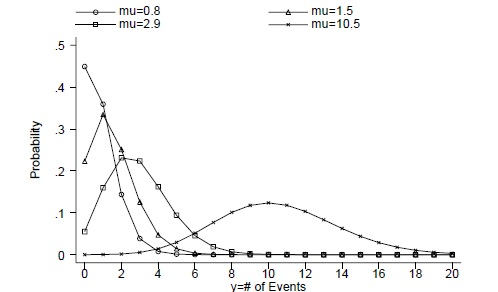
\includegraphics[height=6cm]{1}
% \end{center}

% La trama muestra cuatro características de la distribución de Poisson que son importantes para la comprensión modelos de regresión para el recuento:
% \begin{itemize}
% \item  $\mu$ es la media de la distribución. Como  $\mu$  aumenta, la masa de la distribución se desplaza hacia la derecha.
%  \item $\mu$ es también la varianza. Por lo tanto, $Var (y) = \mu$, que se conoce como equidispersión. En los datos reales, muchas variables de recuento tienen una varianza mayor que la media, que se llama sobredispersión.
%  \item Como $\mu$ aumenta, la probabilidad de que un cero disminución de los recuentos. Para muchas variables de recuento, hay ceros que las predichas por la distribución de Poisson más observado.
%  \item Como $\mu$ aumenta, la distribución de Poisson se aproxima a una distribución normal. Esto se muestra por la distribución de $\mu = 10,5$.
%  \end{itemize}

% \section{Modelo de Regresión de Poisson}\index{Modelo de Regresión de Poisson}

% El modelo de regresión de Poisson (PRM) se extiende de la distribución de Poisson al permitir que cada observación tener un valor diferente de $\mu$. Más formalmente, el PRM asume que el recuento observado para la observación i se extrae de una distribución de Poisson con $\mu_{i}$ de media, donde $\mu_{i}$  se estima a partir  de las características observadas. Esto se refiere a veces como la incorporación de heterogeneidad observada, y conduce a la ecuación estructural:
% \\
% \begin{equation}
% \mu_{i}  =E(y_{i}|x_{i})=exp(x_{i}\beta )
% \end{equation}

% Por lo tanto la distribución de Possion con la variables explicativas x, seria:
% \begin{equation}
% Pr(y | x) =\frac{{e}^{\mu_{i} }\mu_{i}^{y }}{y!}
% \end{equation}
% Tomando el exponencial de  $x\beta$ para  $\mu$ debe ser positivo, lo cual  necesario ya que el conteo sólo puede ser 0 o positivo. Para ver cómo funciona esto, considere el modelo de regresión de Poisson con una sola variable independiente $\mu$ =exp ($\alpha$ $+$ $\beta x$), que puede ser trazada como:

% \begin{center}
% 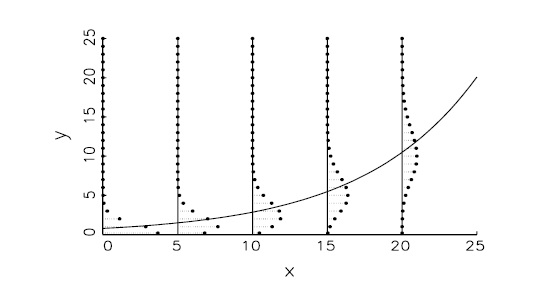
\includegraphics[height=6cm]{2}
% \end{center}

% En este gráfico, la media  $\mu$, que se muestra por la línea curva, aumenta a medida que aumenta x. Para cada valor de  $\mu$, la distribución alrededor de la media se muestra por los puntos y que representan la probabilidad de cada conteo. Interpretación del modelo implica evaluar cómo los cambios en las variables independientes afectan a la media condicional y las probabilidades de varios conteos.

% \subsection{Estimación por máxima verosimilitud }
% \begin{equation}
% lnt =\sum_{i=1}^{n}({-\mu+yln\mu-ln(y!)})
% \end{equation}
% \begin{equation}
% lnt=\sum_{i=1}^{n}({-e^{x\beta}+yx\beta-ln(y!)})
% \end{equation}

% Derivamos la ecuación respecto de $\beta$
% \begin{equation}
% \frac{\partial lnt }{\partial \beta}=\sum_{i=1}^{n}({-xe^{x\beta}+yx})=0
% \end{equation}
% \begin{equation}
% \sum_{i=1}^{n}({xe^{x\beta}})=\sum_{i=1}^{n}{(y_{i}x_{i}})
% \end{equation}

% \begin{equation}
% \frac{\partial^2 lnt }{\partial \beta^2}= -\sum_{i=1}^{n}({xxe^{x\beta}})
% \end{equation}

% \section{Ejemplo de una estimación del modelo de regresión de Poisson en Stata}\index{Ejemplo de una estimación del modelo de regresión de Poisson en Stata}

% Para este ejemplo, utilizamos datos de Long (1990) sobre el número de publicaciones producido por Ph.D. bioquímicos. Las variables consideradas son\\
% . use couart2, clear\\
% . describe\\

% \begin{center}
% \includegraphics[height=4.5cm]{3}
% \end{center}

% . summarize\\

% \begin{center}
% 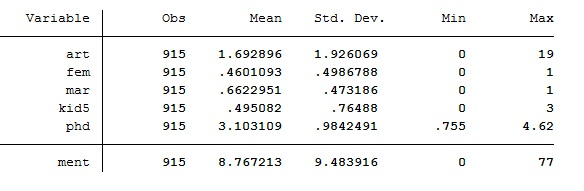
\includegraphics[height=5cm]{4}
% \end{center}

% Las diferencias entre los científicos en sus índices de productividad podría deberse a factores como el género, el estado civil, el número de jóvenes niños, el prestigio del programa de postgrado, y el número de artículos escritos por el mentor de un científico. Para dar cuenta de estas diferencias, añadimos estas variables como variables independientes, donde la variable dependiente sera el numero de artículos en los  últimos 3 años de doctorado.
% \\\\
% Ahora utilizaremos el siguiente comando para estimar el modelo.\\
% . poisson art fem mar kid5 phd ment, nolog\\

% \begin{center}
% 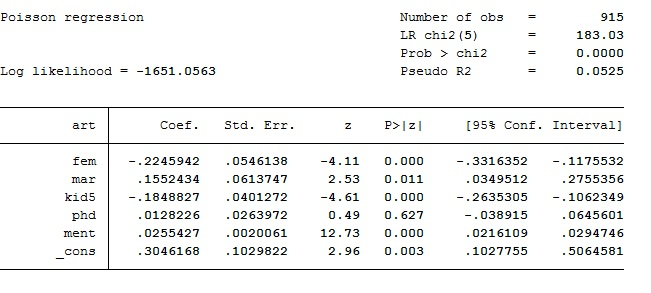
\includegraphics[height=6cm]{5}
% \end{center}

% La manera  en la cual se interpreta  un modelo de conteo depende si se está interesado en el valor esperado de la variable de recuento o en la distribución de los recuentos. Si el interés está en el recuento esperado, varios métodos se pueden utilizar para calcular el cambio en la expectativa de un cambio en una independiente variable.
% \\
% Si el interés está en la distribución de los recuentos o tal vez sólo la probabilidad de que un recuento específico, la probabilidad de que un recuento para un nivel dado de las variables independientes se puede calcular.
% \begin{itemize}
%  \item Factor de Cambio en la E (y / x)\\
% Quizás el método más común de interpretación es el factor de cambio en la tarifa. Si definimos
% E (y / x,$ x_{k}$) como el recuento esperado para un determinado x donde notamos explícitamente el valor de $x_{k}$, y definir E (y / x, $x_{k}$ + $\delta$) como el recuento de espera después de aumentar$ x_{k}$ por unidades $\delta$, entonces
% \begin{equation}
% \frac{E (y / x, x_{k}+ \delta)}{E (y / x, x_{k})}=e^{\beta_{k}\delta}
% \end{equation}
% Por lo tanto, los parámetros pueden ser interpretados como
% Para un cambio de $\delta$ en $x_{k}$, el recuento esperados aumenta en un factor de $exp(\beta_{k}\delta)$, teniendo a  todas las otras variables constantes.
%  \item Cambio porcentual en el E (y / x)\\
% Por otra parte, el porcentaje de cambio en el recuento esperado para un cambio unitario $\delta$ en  $x_{k}$, la celebración de otra las variables constantes, se puede calcular como:

% \begin{equation}
% 100*\frac{E (y / x, x_{k}+ \delta)-E (y / x, x_{k})}{E (y / x, x_{k})}= 100*[exp (\beta_{k}*\delta) - 1]
% \end{equation}
% \end{itemize}
% \subsubsection{Calculamos el factor y el cambio en el E (y / x)}
% Coeficientes de cambio Factor se pueden calcular utilizando listcoef:\\
% . poisson art fem mar kid5 phd ment, nolog\\
% . listcoef fem ment, help\\

% \begin{center}
% 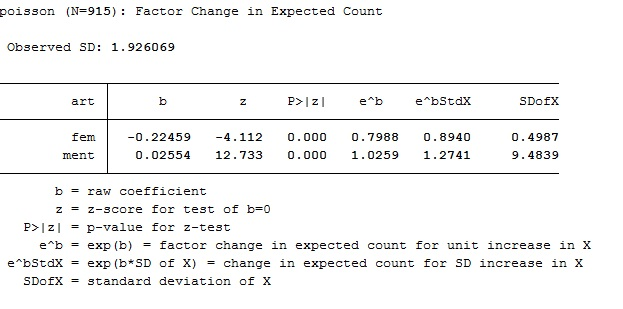
\includegraphics[height=6cm]{6}
% \end{center}

% Por ejemplo, los coeficientes de fem y ment pueden ser interpretados como: Ser una científica disminuye el número esperado de artículos por un factor de 0.80, manteniendo  las demás variables constantes.
% \\
% Para un aumento de una desviación estándar de la productividad del mentor, aproximadamente 9,5 artículos, un medias aumento de la productividad del científico por un factor de 1,27, manteniendo constante otras variables.Para calcular el porcentaje de cambio utilizamos el comando:

% listcoef fem ment, percent help\\

% \begin{center}
% 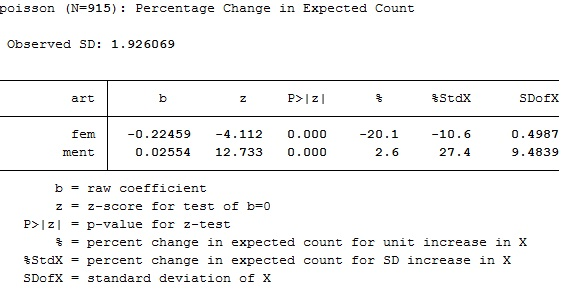
\includegraphics[height=6cm]{7}
% \end{center}

% Por ejemplo, los coeficientes de variación porcentual de fem y ment pueden ser interpretados como:\\
% Ser una científica disminuye el número esperado de artículos en un 20 por ciento, manteniendo todas las otras variables constantes. Por cada artículo adicional por parte del mentor, predijo de un científico de la productividad media aumenta en un 2,6 por ciento, manteniendo constantes otras variables.
% \subsubsection{Cambio marginal en E (y / x)}
% Otro método de interpretación es el cambio marginal en  E (y / x)
% \begin{equation}
% \frac{\partial E (y /  x_{k})}{\partial  x}=E (y / x)\beta_{k}
% \end{equation}
% Para $\beta_{k}> 0$ es  mayor  el valor actual de E (y | x), mayor es la tasa de cambio; para $\beta_{k} <0$,es menor es la tasa de cambio. El marginal respecto de $x_{k}$ depende tanto $\beta_{k}$ y E (y/ x).
% Por lo tanto, el valor de la marginal depende de los niveles de todas las variables en el modelo. En la práctica, este medida a menudo se calcula con todas las variables se encuentren en su medio.
% \subsubsection {Ejemplo de cambio marginal utilizando mfx compute}
% Por default, mfx compute calcula el cambio marginal con variables se encuentren en su medio:\\
% . mfx compute\\

% \subsection{Interpretación utilizando probabilidades predichas}
% Los parámetros estimados se pueden utilizar también para calcular probabilidades predichas utilizando la siguiente fórmula:
% \begin{equation}
% \widehat{Pr}(y =m| x) =\frac{{e}^{-x \widehat{\beta}}({{x \widehat{\beta}}})^{m }}{m!}
% \end{equation}
% Probabilidades pronosticadas en los valores especificados se pueden calcular utilizando prvalue. Las predicciones de los valores observados  para todas las observaciones se pueden calcular usando prcounts.\\
% . poisson art fem mar kid5 phd ment, nolog\\
% . prcounts prm, plot max(9)\\
% . d prm*\\

